\documentclass[compress]{beamer}
\usefonttheme{professionalfonts}



%

\usepackage[T1]{fontenc}
%\usepackage{kmath,kerkis}
%\usepackage{fouriernc}
\usepackage[adobe-utopia]{mathdesign}
%\usepackage{arev}
\usepackage{times}
\usepackage{natbib}

\usepackage[noend]{algpseudocode}
\usepackage{xmpmulti}
\usepackage{dsfont}
\usepackage{amsmath}

\usepackage{graphicx,float,wrapfig, bbm}
\usepackage{amsfonts, comment, bbold}
\usepackage{mdwlist}
\usepackage{subfigure}
\usepackage{colortbl}
\usepackage{mathrsfs}


\usepackage{multirow}




% packages

\usepackage{amsfonts}

% environments

\newenvironment{packed_enumerate}{
  \begin{enumerate}
    \setlength{\topsep}{0pt}
    \setlength{\itemsep}{2pt}
    \setlength{\parskip}{0pt}
    \setlength{\parsep}{0pt}
}{\end{enumerate}}

\newenvironment{stepit}
 {\begin{itemize}[<+-|alert@+>]}
   {\end{itemize}}

% commands

\newcommand{\Norm}[3]{\mathcal{N}\left( #1, #2, #3 \right)}
\newcommand{\popshow}[2]{\only<#1->{\alert<#1>{#2}}}
\newcommand{\x}{\mathbf{x}}
\newcommand{\ex}[1]{\mbox{exp}\left\{ #1\right\} }
\newcommand{\e}[2]{\mathbb{E}_{#1}\left[ #2 \right] }
\newcommand{\g}{\, | \,}
\newcommand{\indpt}{\protect\mathpalette{\protect\independenT}{\perp}}
\def\independenT#1#2{\mathrel{\rlap{$#1#2$}\mkern2mu{#1#2}}}
\newcommand{\E}{\textrm{E}}
\newcommand{\R}{\textrm{R}}
\newcommand{\realline}{\mathbb{R}}
\newcommand{\data}{{\cal D}}
\newcommand{\loglik}{{\cal L}}
\newcommand{\grad}[2]{ \frac{\partial{#1}}{\partial#2}}
\newcommand{\dir}[1]{\mbox{Dir}(#1)}
\newcommand{\mult}[1]{\mbox{Mult}( #1)}
\newcommand{\G}[1]{\Gamma \left( \textstyle #1 \right)}
\newcommand{\ind}[1]{\mathds{1}\left[ #1 \right] }
\newcommand{\norm}[1]{\left\lVert#1\right\rVert}

\newcommand{\class}[1]{ \texttt{#1}}
\newcommand{\term}[1]{ ``#1''}
\newcommand{\tcword}[0]{ w }
\newcommand{\docsetlabeled}[0]{ D }
\newcommand{\onedoclabeled}[0]{ d }
\newcommand{\tcposindex}[0]{ i }
\newcommand{\myblue}[1]{ {\textbf #1 }}
\newcommand{\dnrm}[1]{ _{\mbox{\textsc{ #1 }}}}
\newcommand{\argmax}[0]{ \arg \max }
\newcommand{\tcjclass}[0]{c_j}
\newcommand{\maths}[1]{ {\bf #1}}




% complexity
\renewcommand{\O}{\mathcal{O}}



\setbeamersize{text margin left=0.5cm}
\setbeamersize{text margin right=0.5cm}
\setbeamercolor{alert}{fg=red!75!black}

\usetheme{default}
\useinnertheme{circles}
\useoutertheme{split}
\usecolortheme{seahorse}
% \usecolortheme{dove}
% \usecolortheme{seagull}
%\usecolortheme{default}
% \usecolortheme{dolphin}
\usefonttheme{structurebold}
%\usefonttheme{serif}

\setbeamertemplate{navigation symbols}{}
\setbeamertemplate{headline}{}
\setbeamertemplate{footline}{}
\setbeamerfont{itemize/enumerate subbody}{size=\normalsize}
\setbeamerfont{itemize/enumerate subsubbody}{size=\normalsize}
\setbeamercolor{itemize item}{fg=gray}
\setbeamercolor{enumerate item}{fg=gray}
\setbeamercolor{itemize item}{fg=gray}
\setbeamercolor{itemize subitem}{fg=gray}
\setbeamercolor{item projected}{bg=gray}
\setbeamercolor{subitem projected}{bg=gray}


\newenvironment{bullets}
{\begin{itemize} \setlength{\itemsep}{10pt}}
{\end{itemize}}

\newcommand{\mygraphic}[2]{
  \begin{beamercolorbox}[colorsep*=4pt]{black math}
    \begin{center}
      \includegraphics[#1]{#2}
    \end{center}
  \end{beamercolorbox}
}

\setbeamercolor{structure}{bg=gray}
\setbeamercolor{section in head/foot}{bg=gray}
\setbeamercolor{palette primary}{bg=lightgray}


\usepackage{minted}

\usetheme[pageofpages=of,                    % String used between the current page and the
                                             % total page count.
          bullet=circle,                     % Use circles instead of squares for bullets.
          titleline=true,                    % Show a line below the frame title.
          showdate=true,                     % show the date on the title page
          alternativetitlepage=true,         % Use the fancy title page.
          titlepagelogo=../../common/culogo,              % Logo for the first page.
          % Logo for the header on first page.
          headerlogo=../../common/boulder_cs,
          ]{UCBoulder}

\usecolortheme{ucdblack}
\author{Introduction to Data Science Algorithms}


\institute[Boyd-Graber and Paul] % (optional, but mostly needed)
{Jordan Boyd-Graber and Michael Paul}


\AtBeginSection[] % "Beamer, do the following at the start of every section"
{ \begin{frame} \frametitle{Outline} % make a frame titled "Outline"
\tableofcontents[currentsection] % show TOC and highlight current section
\end{frame} }


\usepackage{amsmath}
\usepackage{bm}

\newcommand{\gfx}[2]{
\begin{center}
	\includegraphics[width=#2\linewidth]{dpmm/#1}
\end{center}
}
\title{Bayesian Non-Parametrics}
\date{Overview}

\begin{document}


\frame{\titlepage
}


\begin{frame}{Clustering as Probabilistic Inference}
	\begin{itemize}
		\item GMM is a probabilistic model (unlike $K$-means)
		\item There are several latent variables:
		\begin{itemize}
			\item Means
			\item Assignments
			\item (Variances)
		\end{itemize}
		\pause
		\item Corresponds to representation in unbounded space
	\end{itemize}
\end{frame}

\begin{frame}{Nonparametric Clustering}

	\begin{itemize}
		\item What if the number of clusters is not fixed?
		\item Nonparametric: can grow if data need it
		\item Probabilistic distribution over number of clusters
	\end{itemize}

\end{frame}



\begin{frame}{Dirichlet Process}

\begin{itemize}
	\item Distribution over distributions
	\item Parameterized by: $\alert<2>{\alpha}, \alert<3>{G}$
	\item<2-> Concentration parameter
	\item<3-> Base distribution
	\item<4-> You can then draw observations from $x \sim $DP$(\alpha, G)$.
\end{itemize}

\end{frame}


\begin{frame}{Defining a DP}

	\begin{itemize}
		\item Break off sticks
                  \begin{align}
                    V_1, V_2, & \dots \sim_{\mbox{iid}} \mbox{Beta}(1,
                    \alpha) \\
                    C_k & \equiv V_k \prod_{j=1}^{k-1} (1 - V_k)
                  \end{align}
		\pause
		\item Draw atoms
                  \begin{equation}
                    \Phi_1, \Phi_2, \dots \sim_{\mbox{iid}} G
                  \end{equation}
		\pause
		\item Merge into complete distribution
                  \begin{equation}
                    \Theta = \sum_k C_k \delta_{\Phi_k}
                  \end{equation}
	\end{itemize}

\end{frame}

\begin{frame}{Properties of a DPMM}

	\begin{itemize}
		\item Expected value is the same as base distribution
		\begin{equation}
			\e{\mbox{DP}(\alpha, G)}{x} = \e{G}{x}
		\end{equation}
		\item As $\alpha \rightarrow \infty$, $\mbox{DP}(\alpha, G) = G$
		\item Number of components unbounded
		\item Impossible to represent fully on computer (truncation)
		\item You can nest DPs
	\end{itemize}

\end{frame}

\begin{frame}{Effect of scaling parameter $\alpha$}

	\gfx{dp-alpha}{.9}

\end{frame}


\begin{frame}{DP as mixture Model}

	\gfx{dp-mixture}{.9}

\end{frame}

\begin{frame}{The Chinese Restaurant as a Distribution}

	To generate an observation, you first sit down at a table.  You sit down at a table proportional to the number of people sitting at the table.
	\begin{center}
	\begin{tabular}{ccc}
	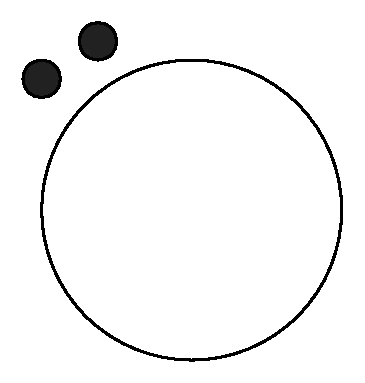
\includegraphics[width=.2\linewidth]{dpmm/table_2} &
	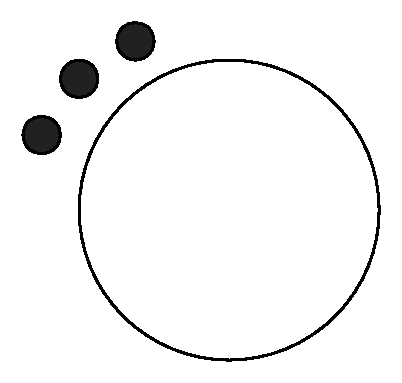
\includegraphics[width=.2\linewidth]{dpmm/table_3} &
         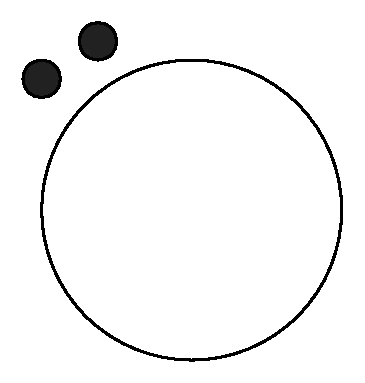
\includegraphics[width=.2\linewidth]{dpmm/table_2} \\
	 \pause
	 $\frac{2}{7}$ & $\frac{3}{7}$ & \alert<3->{$\frac{2}{7}$} \\
	 \pause
	 \pause
	 $x \sim \mu_1$ & $x \sim \mu_2$ & \alert<4>{$x \sim \mu_3$} \\
	\end{tabular}
	\pause
	\begin{block}{But this is just Maximum Likelihood}
		Why are we talking about Chinese Restaurants?
	\end{block}
	\end{center}

\end{frame}

\begin{frame}{Always can squeeze in one more table \dots}

	\begin{itemize}
		\item The \emph{posterior} of a DP is CRP
		\item A new observation has a new table / cluster with probability proportional to $\alpha$
		\item But this must be balanced against the probability of an observation \emph{given a cluster}
                  \begin{equation}
                    \Theta = \sum_k C_k \delta_{\Phi_k}
                  \end{equation}

	\end{itemize}

\end{frame}


\begin{frame}{Gibbs Sampling}

	\begin{itemize}
		\item We want to know the cluster assignment of each observation \only<4->{(tables)}
		\item Take a random guess initially
		\pause
		\item This provides a mean for each cluster
		\pause
		\item Let the number of clusters grow
	\end{itemize}

\end{frame}

\begin{frame}{Gibbs Sampling}

	\begin{itemize}
		\item We want to know $\vec z$
		\item Compute $p(z_i \g z_1 \dots z_{i-1}, z_{i+1}, \dots z_m, x, \alpha, G)$
		\item Update $z_i$ by sampling from that distribution
		\item Keep going \dots
	\end{itemize}
	\pause
	\begin{block}{Notation}
		\begin{equation}
			p(z_i = k \g z_{-i}) \equiv p(z_i \g z_1 \dots z_{i-1}, z_{i+1}, \dots z_m)
		\end{equation}
	\end{block}
\end{frame}

\begin{frame}{Gibbs Sampling for DPMM}

	\begin{align}
		& p(z_i =k \g \vec z_{-i}, \vec x, \{\theta_k\}, \alpha) \\
\only<2->{		= & p(z_i = k \g \vec z_{-i}, x_i, \vec x, \theta_k, \alpha) \\}
\only<3->{		= & p(z_i = k \g \vec z_{-i}, \alpha) p(x_i \g \theta_k, \vec x) \\}
\only<4->{		= & \begin{cases} \left( \frac{n_k}{n_\cdot + \alpha} \right) \int_\theta p(x_i \g \theta) p(\theta \g G, \vec x) & \mbox{existing} \\
		\frac{\alpha}{n_\cdot + \alpha} \int_\theta p(x_i \g \theta) p(\theta \g G) & \mbox{new} \end{cases} \\}
\only<5->{		= & \begin{cases} \left( \frac{n_k}{n_\cdot + \alpha} \right) \Norm{x}{\frac{n \bar{x}}{n + 1}}{\mathbb{1}} & \mbox{existing} \\
		\frac{\alpha}{n_\cdot + \alpha} \Norm{x}{0}{\mathbb{1}}  & \mbox{new} \end{cases}		}
	\end{align}

\only<2>{Dropping irrelevant terms}
\only<3>{Chain rule}
\only<4>{Applying CRP}
\only<5>{Scary integrals assuming $G$ is normal distribution with mean zero and unit variance.  (Derived in optional reading.)}

\end{frame}


\begin{frame}{Algorithm for Gibbs Sampling}

\begin{enumerate}
	\item Random initial assignment to clusters
	\item For iteration $i$:
	\begin{enumerate}
		\item ``Unassign'' observation $n$
		\item Choose new cluster for that observation
	\end{enumerate}
\end{enumerate}

\end{frame}



\end{document}
